\documentclass[fontsize=12pt]{article}

\usepackage{amsmath}
\usepackage[utf8]{inputenc}
\usepackage[margin=0.75in]{geometry}
\usepackage[labelformat=empty]{caption}
\usepackage{smartdiagram}
\usepackage{multirow}
\usepackage[edges]{forest}
\usepackage{graphicx}
\usepackage{lipsum}
\usepackage[dvipsnames]{xcolor}
\usepackage{caption}
\usepackage{subcaption}
\usepackage[
    backend=bibtex,
    isbn=false,
    url=false,
    doi=false,
    eprint=false,
]{biblatex}
\definecolor{foldercolor}{RGB}{241,213,146}

\tikzset{pics/folder/.style={code={%
    \node[inner sep=0pt, minimum size=#1](-foldericon){};
    \node[folder style, inner sep=0pt, minimum width=0.3*#1, minimum height=0.6*#1, above right, xshift=0.05*#1] at (-foldericon.west){};
    \node[folder style, inner sep=0pt, minimum size=#1] at (-foldericon.center){};}
    },
    pics/folder/.default={20pt},
    folder style/.style={draw=foldercolor!80!black,top color=foldercolor!40,bottom color=foldercolor}
}

\forestset{is file/.style={edge path'/.expanded={%
        ([xshift=\forestregister{folder indent}]!u.parent anchor) |- (.child anchor)},
        inner sep=1pt},
    this folder size/.style={edge path'/.expanded={%
        ([xshift=\forestregister{folder indent}]!u.parent anchor) |- (.child anchor) pic[solid]{folder=#1}}, inner ysep=0.6*#1},
    folder tree indent/.style={before computing xy={l=#1}},
    folder icons/.style={folder, this folder size=#1, folder tree indent=3*#1},
    folder icons/.default={12pt},
}
\title{%
  CSC111 Course Project Report \\
  \large Stockify App}

\author{Mahe Chen, Aarya Bhardawaj, Matthew Yu and Daniel Cheng}
\date{April 1, 2023}

\begin{document}
\maketitle

\section*{Problem Description and Research Question}

\begin{itemize}
\item

\textbf{Background and Overview}

\end{itemize}

\begin{quote}
\noindent \textit{“You pay a very high price in the stock market for a cheery consensus” - Warren Buffet.}

A stock is the division of ownership of a corporation or company through shares. The stock market is a complex network of exchanges where investors and traders buy and sell shares of publicly traded companies (Stock market 101). It has been a traditional source of funding for companies to expand their businesses and for investors to receive dividends in return for sharing ownership of companies. The stock market is a dynamic and ever-changing place where stock values for different companies rise and fall due to various factors. This makes it a potentially profitable but risky investment option. To make the most informed decisions with their money, stock traders often require guidance.
\end{quote}

\begin{itemize}
\item
  
  \textbf{Motivation}
 
\end{itemize}

\begin{quote}
\noindent The stock market offers ample opportunities, yet not everyone takes advantage of them. For many, investing in stocks can be an intimidating prospect, even for seasoned investors. Determining whether a stock is worth investing in is not always straightforward, and predicting its future performance can be challenging. It requires a considerable amount of analysis and investment management to make informed investment decisions.

To assist beginners in navigating the stock market and making sound investment choices, we have designed a program that is specifically tailored for this purpose. Our program allows users to limit their search by stock sector, value, risk, and other characteristics, and provides clear recommendations of the most fitting stock purchases, along with detailed information about these stocks.  

\textbf{Our primary objective is to create an application that recommends optimal stocks based on the user's preferences. Whether you are new to investing or looking for a simpler way to manage your investments, our program is an effective solution that can help you achieve your investment goals.}
\end{quote}

\section*{Computational Plan}
\begin{center}
  \begin{forest}
    for tree={font=\sffamily, %grow'=0,
    folder indent=.9em, folder icons,
    edge=densely dotted}
    [Stockify
      [\textcolor{orange}{data.zip}, 
          [\textcolor{teal}{stock$\_$data.csv}, is file]
          [\textcolor{teal}{stock$\_$symbols.csv}, is file]
          ]
      [\textcolor{blue}{rw$\_$csv.py}, is file]
      [\textcolor{blue}{load$\_$objects.py}, is file]
      [\textcolor{blue}{stock$\_$classes.py}, is file]
      [\textcolor{blue}{decision$\_$computation.py}, is file]
      [\textcolor{blue}{gui.py}, is file]
      [\textcolor{blue}{main.py}, is file]    
    ]
  \end{forest}
\end{center}
\begin{itemize}
\item
  
  \textbf{Dataset: \textcolor{teal}{stock$\_$data.csv, stock$\_$symbols.csv}}
  
\end{itemize}

\begin{quote}
\noindent To create an effective dataset for our stock recommender, we utilized the Python requests library and web scraped data on a total of 3568 stocks from Yahoo Finance. After filtering out stocks with insufficient data, we were left with 3505 stocks. We began by storing a list of all 3505 stock symbols, which were extracted from a CSV file of large cap stocks from the US stock market. Next, we used a function to web scrape relevant stock information for each stock, by iterating over the list of stock symbols and using the requests.get function to change the "stock" portion of the URL. The write$\_$stock$\_$data function recorded all the relevant attributes for each stock and stored this information in a CSV file. This resulted in a dataset containing all 3505 stocks and their respective attributes.

For each stock, we recorded a total of 24 attributes, with most of them being about the company rather than the stock itself. We included information such as debt to equity ratio, return on equity ratio, and profit margins, as these attributes are crucial in evaluating a stock's future potential. We focused on computing 7 scores, value score, growth score, quality score, consistency score, risk score, ESG score, and dividend score using the extracted data. To accomplish this, we implemented a load csv function to read all the data from the generated CSV file and store all the instance attributes for each stock. This was the final step in our data accumulation process. By using this method, we can have up-to-date stock information and easily update our dataset in real-time by running our function again.
\end{quote}
\begin{center}
\begin{tabular}{|p{1.5cm}|p{1.5cm}|p{1.5cm}|p{1.5cm}|p{1.5cm}|p{1.5cm}|p{1.5cm}|p{1.5cm}|}
 \hline
 \multicolumn{8}{|c|}{Sample row of the csv file with the first few headers:} \\
 \hline
symbol & sector & name & address & previous & dividend & high & low\\
 \hline
AAPL & Technology & Apple & Cupertino & 160.77 & 0.0057 & 178.49 & 124.17\\
 \hline
\end{tabular}
\end{center}
\begin{itemize}
\item
  
  \textbf{Data Wrangling: \textcolor{blue}{stock$\_$classes.py}}
 
\end{itemize}
\begin{quote}
\noindent Our program will rely on decision trees to provide the stock recommendations. Each root(excluding the root of the main tree) will hold some question as an attribute. The subtrees for each internal root correspond to the possible answers the decision may branch into. The path taken depends on the user’s answer to that question, with the leaves at the end of the tree representing the resulting stock(s) from taking that path down the tree. This file contains the DecisionTree class and the $\_$StockValue class. The decision tree uses the scaled function to convert all the score attributes into skill attributes. These skill attributes are values from 1 - 3 for each stock. This is used to determine which way to go down the tree based on the user preference. The main recursive function to generate the decision tree is the insert$\_$stock$\_$sequence function. This function adds all the stocks into the decision tree. The $\_$StockValue is a recursive class which holds a stock in a StockGraph. The StockGraph class is a recursive class which contains the last node of the tree. Accessing the neighbours returns a list of all recommended stocks.

The StockScore class is then used to record these respective value scores for each stock. The SectorAverage class is used to record all the data which may have missing values. These are the attributes with an ‘Optional’ type annotation in the StockData class. If these attributes have missing values and are ‘None’, then we will use the get$\_$avg$\_$of$\_$sector function to compute the average value of that respective attribute for all stocks in the same sector as the one with the missing data. This value is then used in the computation in the ‘get score’ functions. 

This file contains the StockData, SectorAverage, and the StockScore classes. The StockData class contains all the attributes extracted from the stock$\_$data.csv file. These attributes are used to compute the 7 scores our stock recommender will use to recommend a stock based on user preferences. This file contains 7 ‘get score’ functions, these are the get$\_$value$\_$score, get$\_$growth$\_$score, getvquality$\_$score, get$\_$consistency$\_$score, get$\_$risk$\_$score, get$\_$esg$\_$score, and get$\_$dividend$\_$score functions. The formulas for each function were created by referencing information from Investopedia and The Motley Fool. The scores are calculated using the following formulas:

\textcolor{blue}{Value score}:

The value score is computed by multiplying the price to earning ratio by the price to book ratio. This will provide an evaluation of the stock based on expectations for future growth and the market value of a company’s shares.

\textcolor{blue}{Growth score}:

The growth score is computed by dividing the earnings before interest, taxes, depreciation, and amortisation by companies sales (ebitda) by the company’s total total sales and then multiplying that value by the companies earnings growth. Dividing ebitda by sales will provide insight on how financially stable a company is and then multiplying by a company's earnings growth will provide insight on how likely the company stock is projected to grow in the near future.

\textcolor{blue}{Quality score}:

The quality score is computed by dividing a company stock's profit margin by its return on equity ratio and then dividing by its debt to equity ratio. This gives a quality score on the stock based on how risky and profitable the company's investments are for that stock.

\textcolor{blue}{Consistency score}:
The consistency score is computed by subtracting the stocks fifty two week high by the fifty two week low, and then dividing by the two hundred day average. This value will give insight on how consistent the stock has been performing over the last fiscal year. A lower score will mean that the stock price is not jumping up or down. 

\textcolor{blue}{Risk score}:

The risk score is computed by dividing the total cash by the current liabilities. This measures how risky it would be to invest in this stock based on the company’s financial status. A higher risk score indicates that the company has significantly higher amounts of current liabilities, short term debt, compared to their total cash at hand. This means the stock has a higher chance of going into
bankruptcy due to insufficient cash.

\textcolor{blue}{ESG score}:

The esg score is computed by taking the average of the company's social score, environmental score, and governance score. By taking the average of a company stocks social, environmental, and governance score, this esg score is able
to represent how well a company is able to address risks with respect to these attributes. A higher esg score means the company is able to effectively address the risk.

\textcolor{blue}{Dividend score}:

The dividend score is directly an attribute of the stock StockData class, thus there is no need to compute this score. The dividend score is simply the dividend yield of a company stock. A high dividend score indicates that the company is returning a lot of its profits to investors. 

\end{quote}

\begin{itemize}
\item
  
  \textbf{Data Computation: \textcolor{blue}{decision$\_$computation.py}}
 
\end{itemize}
\begin{quote}
\noindent Our program will rely on decision trees to provide the stock recommendations. Each root(excluding the root of the main tree) will hold some question as an attribute. The subtrees for each internal root correspond to the possible answers the decision may branch into. The path taken depends on the user’s answer to that question, with the leaves at the end of the tree representing the resulting stock(s) from taking that path down the tree. This file contains the DecisionTree class and the $\_$StockValue class. The decision tree uses the scaled function to convert all the score attributes into skill attributes. These skill attributes are values from 1 - 3 for each stock. This is used to determine which way to go down the tree based on the user preference. The main recursive function to generate the decision tree is the insert$\_$stock$\_$sequence function. This function adds all the stocks into the decision tree. The $\_$StockValue is a recursive class which holds a stock in a StockGraph. The StockGraph class is a recursive class which contains the last node of the tree. Accessing the neighbours returns a list of all recommended stocks.

The StockScore class is then used to record these respective value scores for each stock. The SectorAverage class is used to record all the data which may have missing values. These are the attributes with an ‘Optional’ type annotation in the StockData class. If these attributes have missing values and are ‘None’, then we will use the get$\_$avg$\_$of$\_$sector function to compute the average value of that respective attribute for all stocks in the same sector as the one with the missing data. This value is then used in the computation in the ‘get score’ functions. 
\end{quote}

\begin{center}
\begin{tabular}{ |p{3.5cm}|p{3.5cm}|p{3.5cm}|p{3.5cm}|}
 \hline
 \multicolumn{4}{|c|}{Our Decision Factors:} \\
 \hline
 Stock Value & Stock Growth & Stock Quality & Consistency\\
 \hline
 Social Responsibility & Dividend & Financial Risk & Sectors\\
 \hline
\end{tabular}
\end{center}

\begin{figure}[htbp]
\centering
\begin{minipage}[b]{0.45\textwidth}
\centering
\smartdiagramset{
bubble center node font = \small,
bubble node font = \scriptsize,
bubble center node size =3cm,
bubble node size =2cm,
}
\tikzset{bubble center node/.append style={rotate=0}}
\tikzset{
bubble node/.append style={
text width=1.5cm,
align=center}
}
\smartdiagram[bubble diagram]{
\rotatebox{-0}{Desired Stocks}, AMZN, CEG, CMG, GOOG, LLY, MTCH
}{}
\caption*{StockGraph}
\label{fig:bubble}
\end{minipage}
\hspace{0.05\textwidth}
\begin{minipage}[b]{0.45\textwidth}
\centering
\begin{forest}
for tree={
parent anchor=south,
child anchor=north,
fit=band,
}
[DecisionTree, [V1[G1[...[...[SG]]]][G2[...[...[SG]]]][G3[...[...[SG]]]]][V2[G1[...[...[SG]]]][G2[...[...[SG]]]][G3[...[...[SG]]]]][V3[G1[...[...[SG]]]][G2[...[...[SG]]]][G3[...[...[SG]]]]]]
\end{forest}
\caption*{DecisionTree}
\label{fig:forest}
\end{minipage}
\end{figure}

\begin{center}
Two diagrams that illustrate how DecisionTree Class and StockGraph Class works in our backend.
\end{center}
\newpage
\begin{itemize}
\item
  
  \textbf{Data Visualization: \textcolor{blue}{gui.py}}

\end{itemize}

\begin{quote}
\noindent The user interface is implemented in the \texttt{gui.py} file using the \texttt{Pygame} module. \texttt{Pygame}'s \texttt{Surface} objects and the \texttt{display} module's \texttt{update} method are essential for displaying the interface on the user's screen. In the \texttt{$\_set\_dimension\_variables$} function, the interface adjusts the size of buttons and positions of text according to the user's screen size.

To initialise the buttons for each panel screen, the program uses several initialisation functions. \textcolor{red}{Buttons} are objects that collect user input and trigger the program's response to the input. There are various button classes, each with unique behaviours. For instance, a \textcolor{red}{Checkbox} can be selected to record the user's choices, while a \textcolor{red}{NaviButton} allows the user to navigate between pages when clicked. Specialty buttons, such as the \textcolor{red}{NextStockButton} or \textcolor{red}{SelectAllButton}, have been implemented to tie our user interface to decision tree computations or allow users to select all options with a single click.

Each button uses \texttt{pygame.Rect} objects to represent the button's actual display on the user interface. Additionally, the \texttt{ButtonGroup} class has been created to organise the checkboxes for the select-one page, ensuring only one button is selected for each question.

The contents are displayed on the screen within a continuously running while loop. When a change is made, the program redisplay the contents on the screen. However, during panel transitions, an \texttt{$\_fade\_out$} function has been implemented to display a smoother fade-in and fade-out transition. The \texttt{$get\_pos$} function from the \texttt{pygame.mouse} module helps us determine the user's mouse position, while the \texttt{pygame.event} module allows us to determine when the user left clicks. By combining these two, we can determine when the user clicks on a button and run the button's action method and other program behaviours accordingly.

The program uses modules such as \texttt{pygame.font} and \texttt{pygame.image} to enhance communication and visual appeal. Additionally, functions such as \texttt{$draw\_text$}, \texttt{$\_center\_coordinates$}, and \texttt{$\_split\_str\_to_paragraph$} have been implemented to display nicely formatted and centred text, as well as buttons.

When the program initialises, the user will first be greeted by a loading screen. The \texttt{$\_loading\_screen$} function has been implemented to display loading screens to the user interface anytime the program may take time for computations. From the main menu, the user may start their search, navigate to the instructions or credits panel, or update the stocks in the csv file.

When the user conducts their search, they select their preferences through the checkboxes, and the results containing the recommended stock information are displayed on the results screen. If there are multiple recommended stocks, the user can view each one by clicking the \textcolor{red}{NextStockButton}. The \textcolor{red}{ResetButton} allows the user to clear their search and begin a new one. Finally, the \textcolor{red}{Quit} button allows the user to quit the program anytime.
\end{quote}

\section*{User Instructions}
\begin{itemize}
\item
\textbf{\textcolor{red}{Requirements}}
\end{itemize}
\begin{quote}
\noindent
1. Install all required Python libraries in the requirements.txt file.

2. Download all files in the data.zip file submitted to MarkUs. There should be 3 files inside the folder: stock$\_$data.csv, stock$\_$symbols.csv, and menu$\_$image.jpg.  Save this folder on the same level as the .py files.
\end{quote}
\begin{itemize}
\item
\textbf{\textcolor{red}{Initializing the program}}
\end{itemize}
\begin{quote}
\noindent
1. Open Pycharm and run the main.py file in the Python console.

2. Your screen should be filled with a Pygame screen. This screen may say “Loading…”. Anytime you encounter this screen(a), please be patient - the program takes time to run.
Note: Your screen must be at minimum 1000 x 600 for our program to properly fill the screen. If it is smaller, a 1000 x 600 screen will display(the window will be too large for your screen).
You should eventually be brought to the main screen(b). You have a lot of options here! We’ll briefly explore each one.

Click ‘Instructions’ to be brought to the instructions panel(c). You’ll find a brief description of the program here, as well as definitions for the stock qualities. Click ‘Back’ to return to the main screen.

Click ‘Credits’ to view the credits panel(d). Click ‘Back’ to return to the main screen.

Click ‘Update Stocks’ to update the stock data file to real-time, updated data gathered from Yahoo Finance. You should be brought to a confirmation page(e). 

Click ‘Confirm’ to continue with the process, where you will be greeted with a loading screen and automatically returned to the menu once the process is finished. 

Click ‘Back’ if you instead wish to return to the main screen.

Note: Updating the stocks may take a very long time(10+ minutes). Exiting early will corrupt the csv file.

Click ‘Search’ to begin your search! Walkthrough below.

Click the ‘Quit’ button in the bottom right corner anytime you wish to exit the program.
\end{quote}

\begin{figure}[!htb]
\minipage{0.32\textwidth}
  
\includegraphics[width=\linewidth]{img/a.png}
  \caption{A}\label{fig:awesome_image1}
\endminipage\hfill
\minipage{0.32\textwidth}
  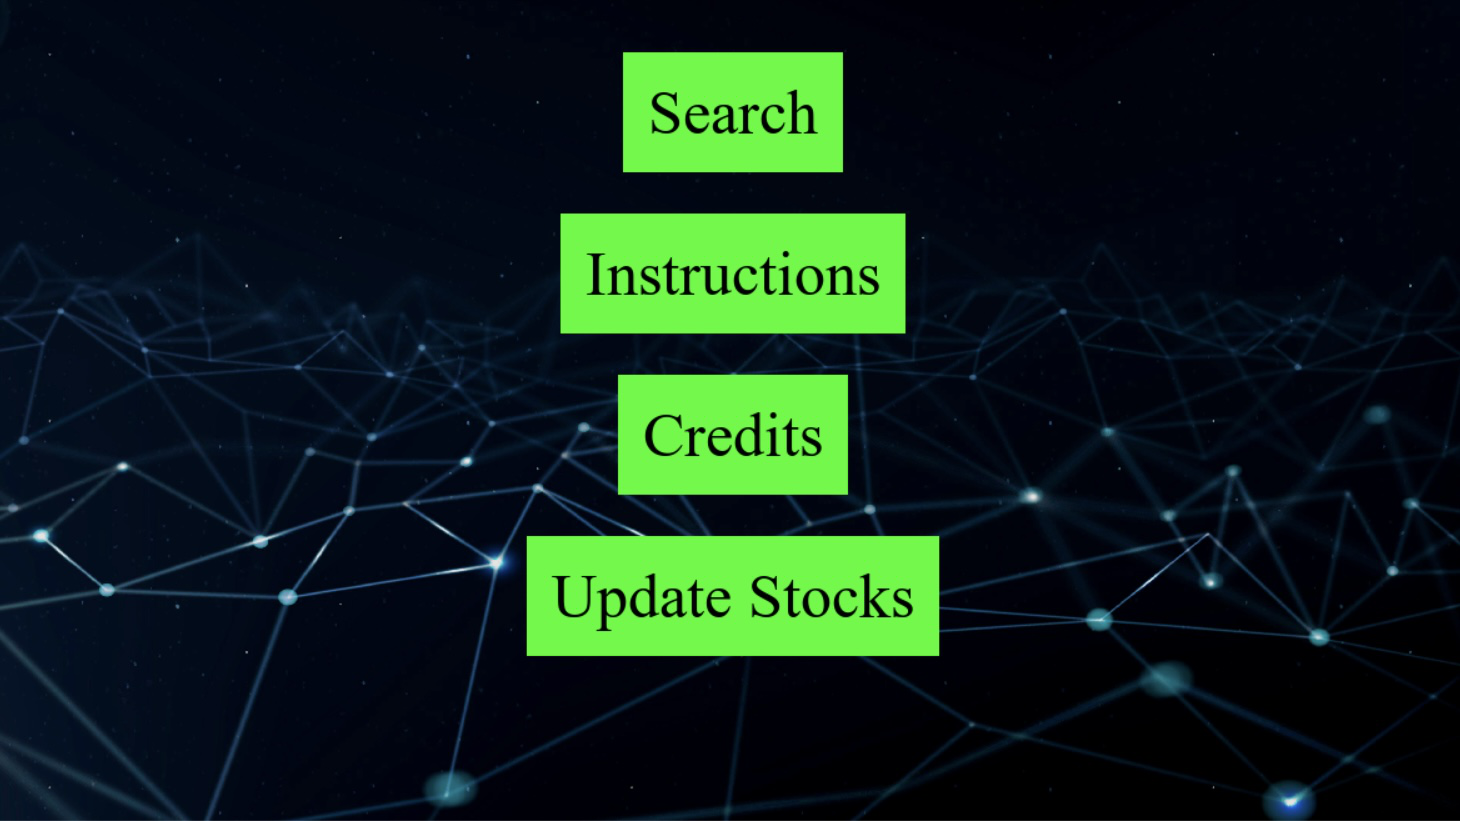
\includegraphics[width=\linewidth]{img/b.png}
  \caption{B}\label{fig:awesome_image2}
\endminipage\hfill
\minipage{0.32\textwidth}%
  
\includegraphics[width=\linewidth]{img/c.png}
  \caption{C}\label{fig:awesome_image3}
\endminipage
\end{figure}

\begin{figure}[!htb]
\minipage{0.32\textwidth}
  
\includegraphics[width=\linewidth]{img/d.png}
  \caption{D}\label{fig:awesome_image1}
\endminipage\hfill
\minipage{0.32\textwidth}
  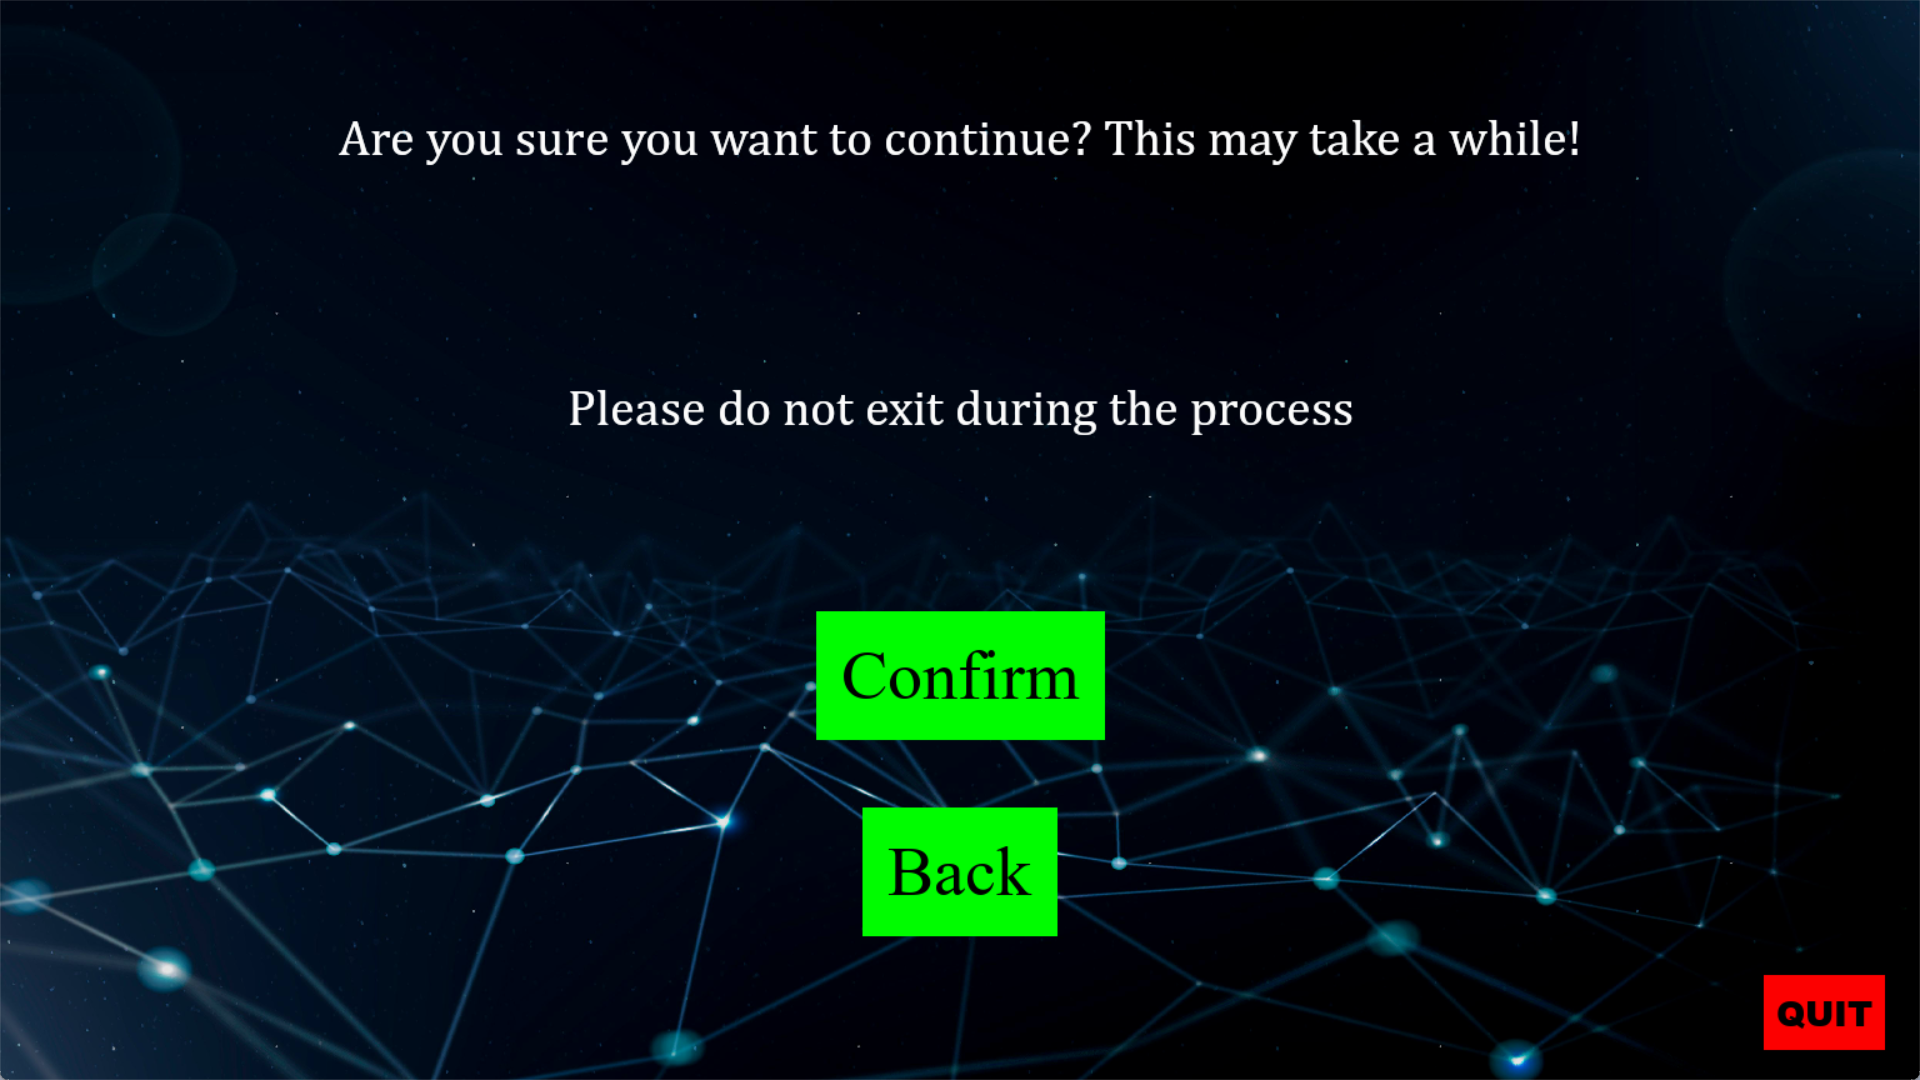
\includegraphics[width=\linewidth]{img/e.png}
  \caption{E}\label{fig:awesome_image2}
\endminipage\hfill
\minipage{0.32\textwidth}%
  
\includegraphics[width=\linewidth]{img/f.jpg}
  \caption{F}\label{fig:awesome_image3}
\endminipage
\end{figure}
\newpage
\begin{itemize}
\item
\textbf{\textcolor{red}{Completing a Search}}
\end{itemize}
\begin{quote}
\noindent
You should first be brought to a screen with a table of checkboxes (f). As indicated by the title, select one checkbox for each row. A checkbox will turn yellow when selected. Once each row has a selection, the ‘Next’ button should become enabled and you can continue on to the next step.

Next, you’ll be brought to another screen with checkboxes and labels(g). As indicated by the title, select the checkbox corresponding to each sector if you wish to receive recommendations for that sector. You can use the ‘Select All’ and ‘Deselect All’ buttons at the bottom of the screen to quickly select or deselect all checkboxes. Now just click ‘Results’ to get your results!

Recommended stock information will be displayed(h). If there are no recommended stocks, then no stocks will be displayed. If there is more than one recommended stock, you can use the arrows in the bottom left corner to navigate between your recommended stocks. Click ‘Restart’ to clear your search and return to the menu.

\end{quote}

\begin{figure}[!htb]
\minipage{0.24\textwidth}
  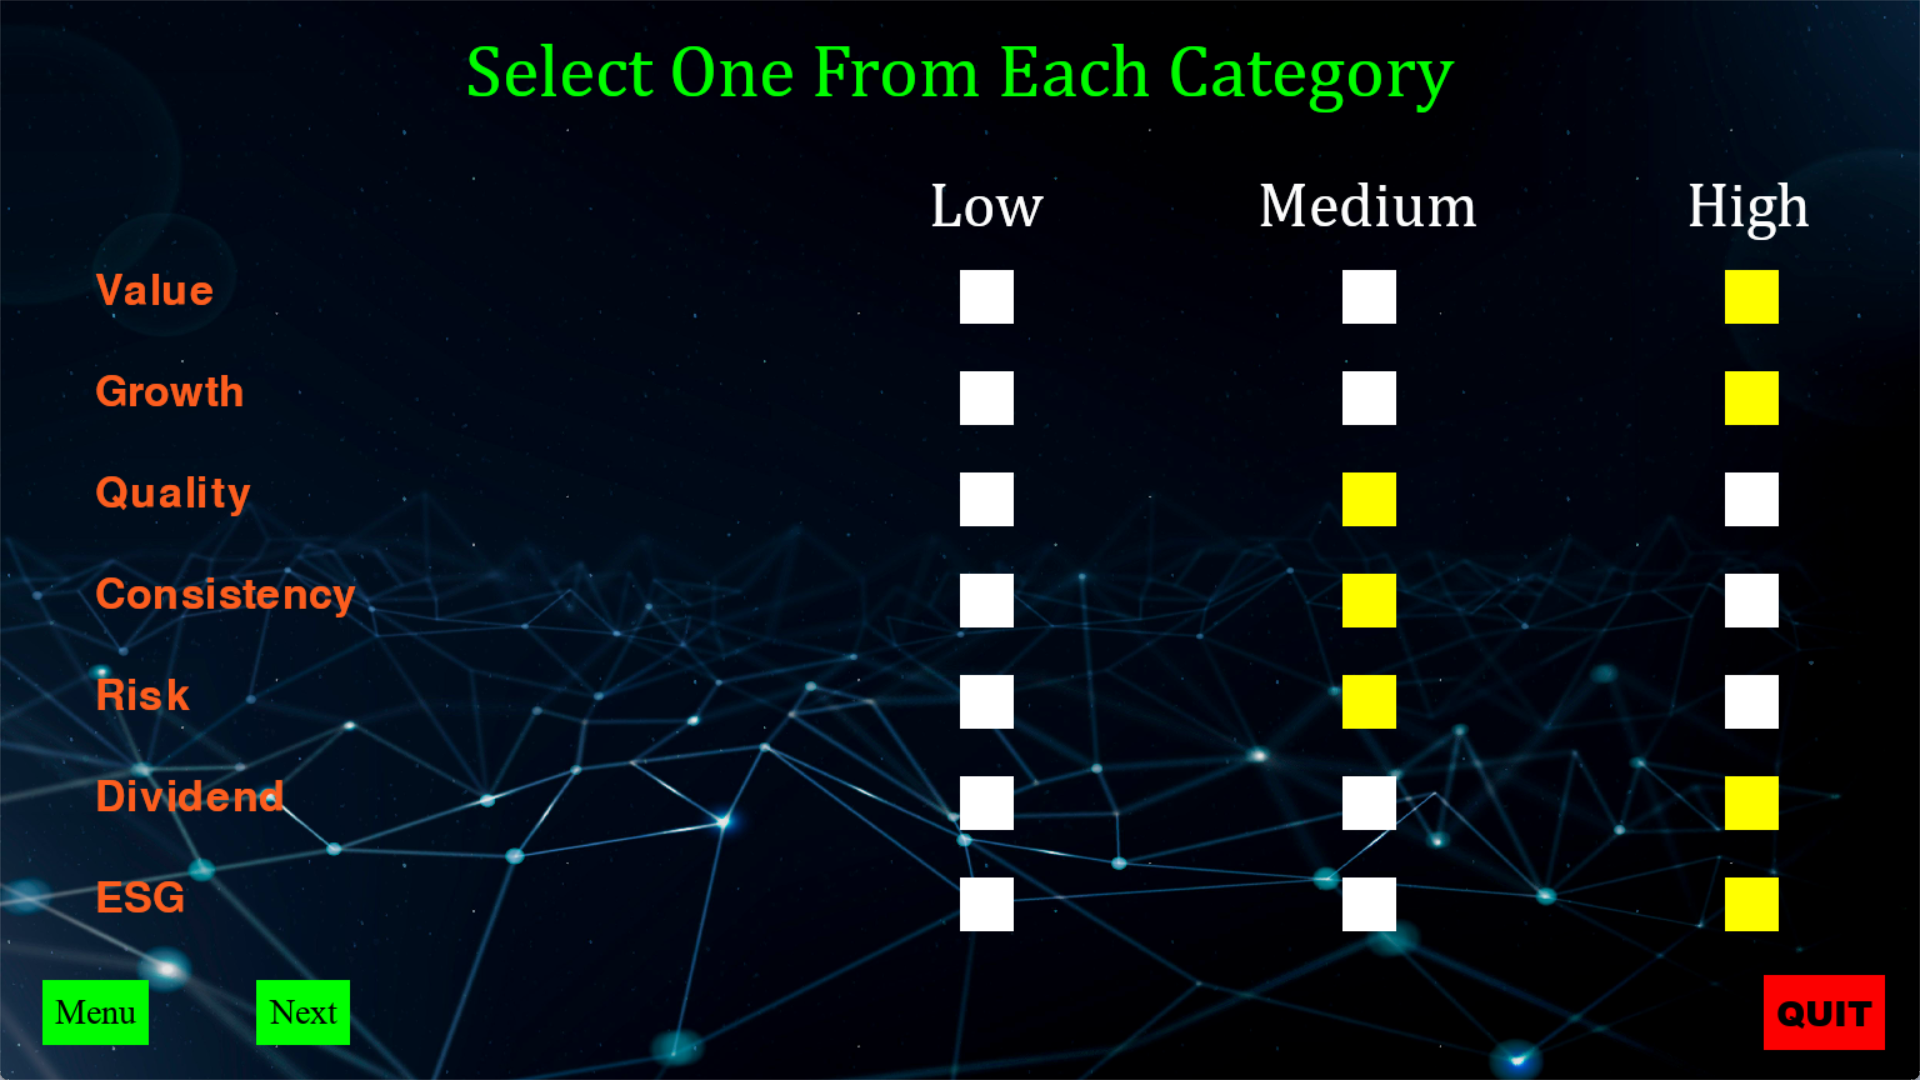
\includegraphics[width=\linewidth]{img/g.png}
  \caption{G}\label{fig:awesome_image1}
\endminipage\hfill
\minipage{0.24\textwidth}
  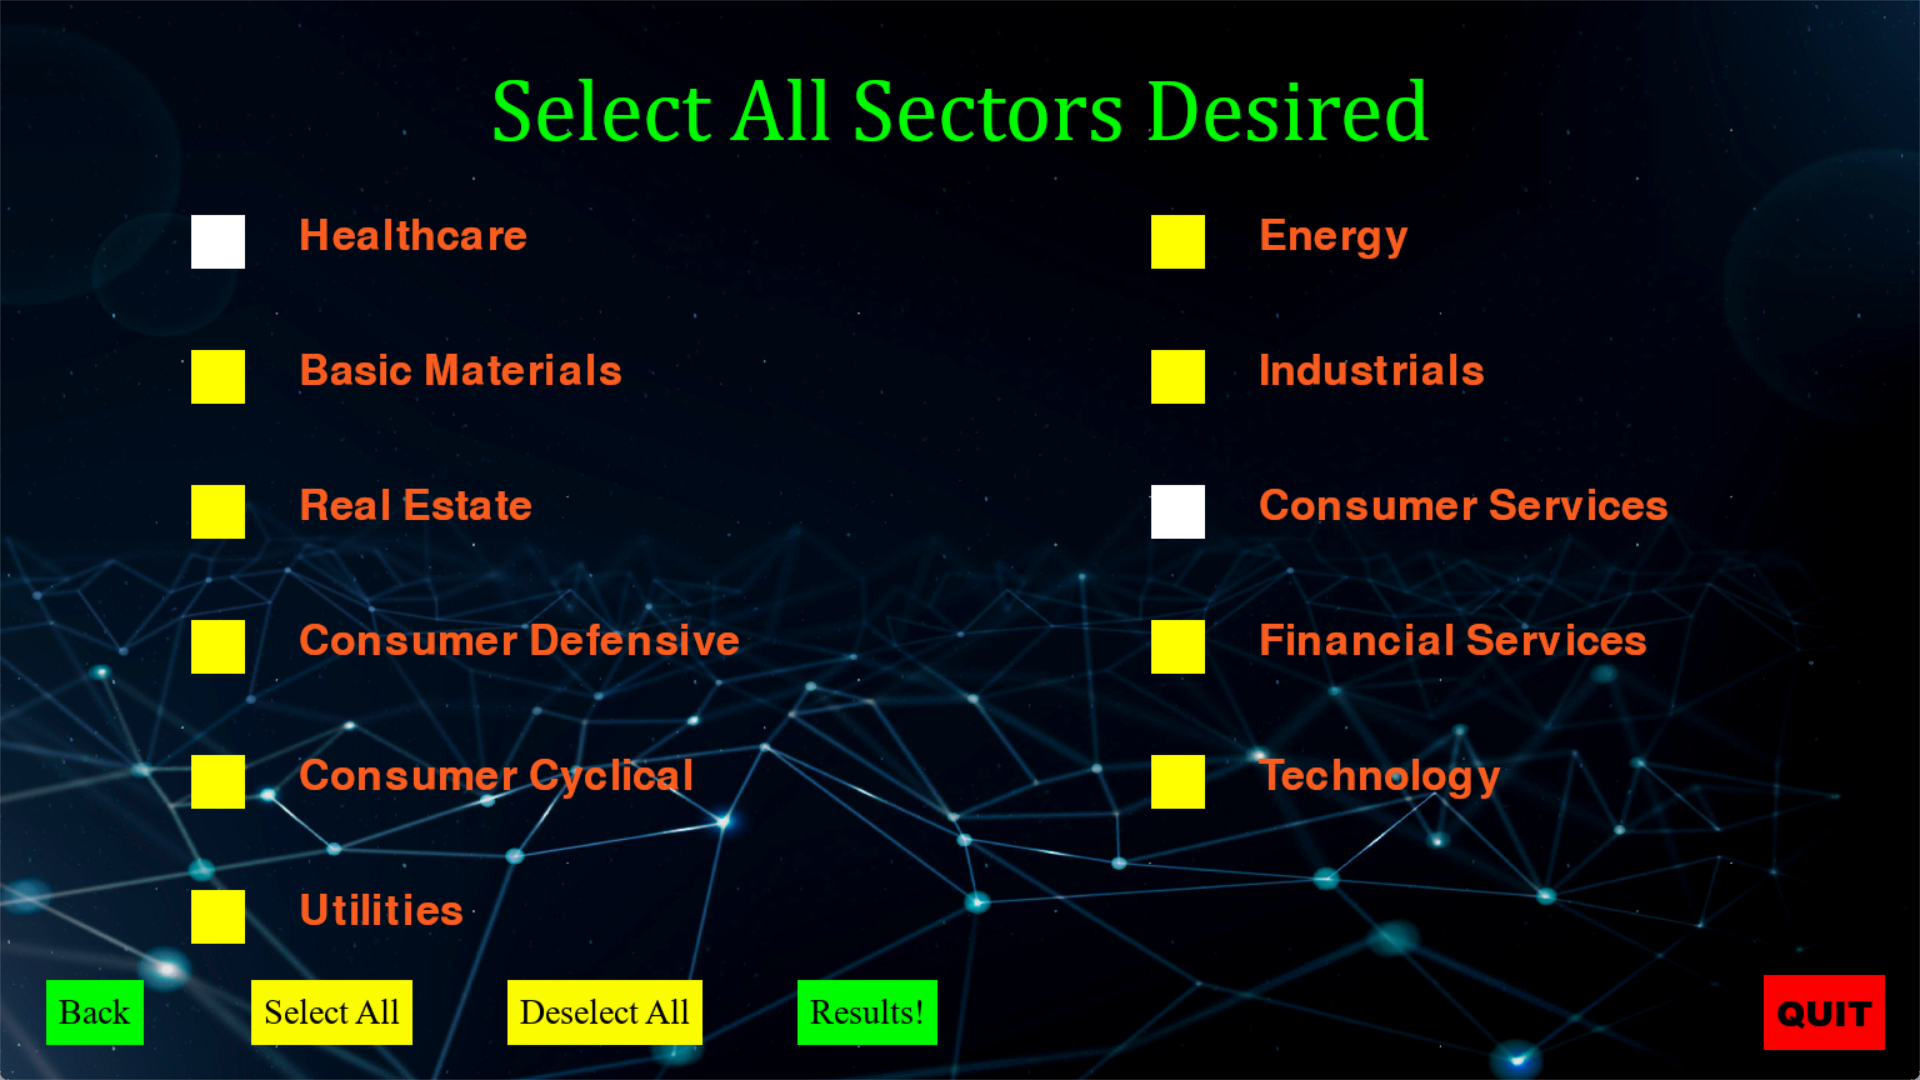
\includegraphics[width=\linewidth]{img/h.png}
  \caption{H}\label{fig:awesome_image2}
\endminipage\hfill
\minipage{0.24\textwidth}
  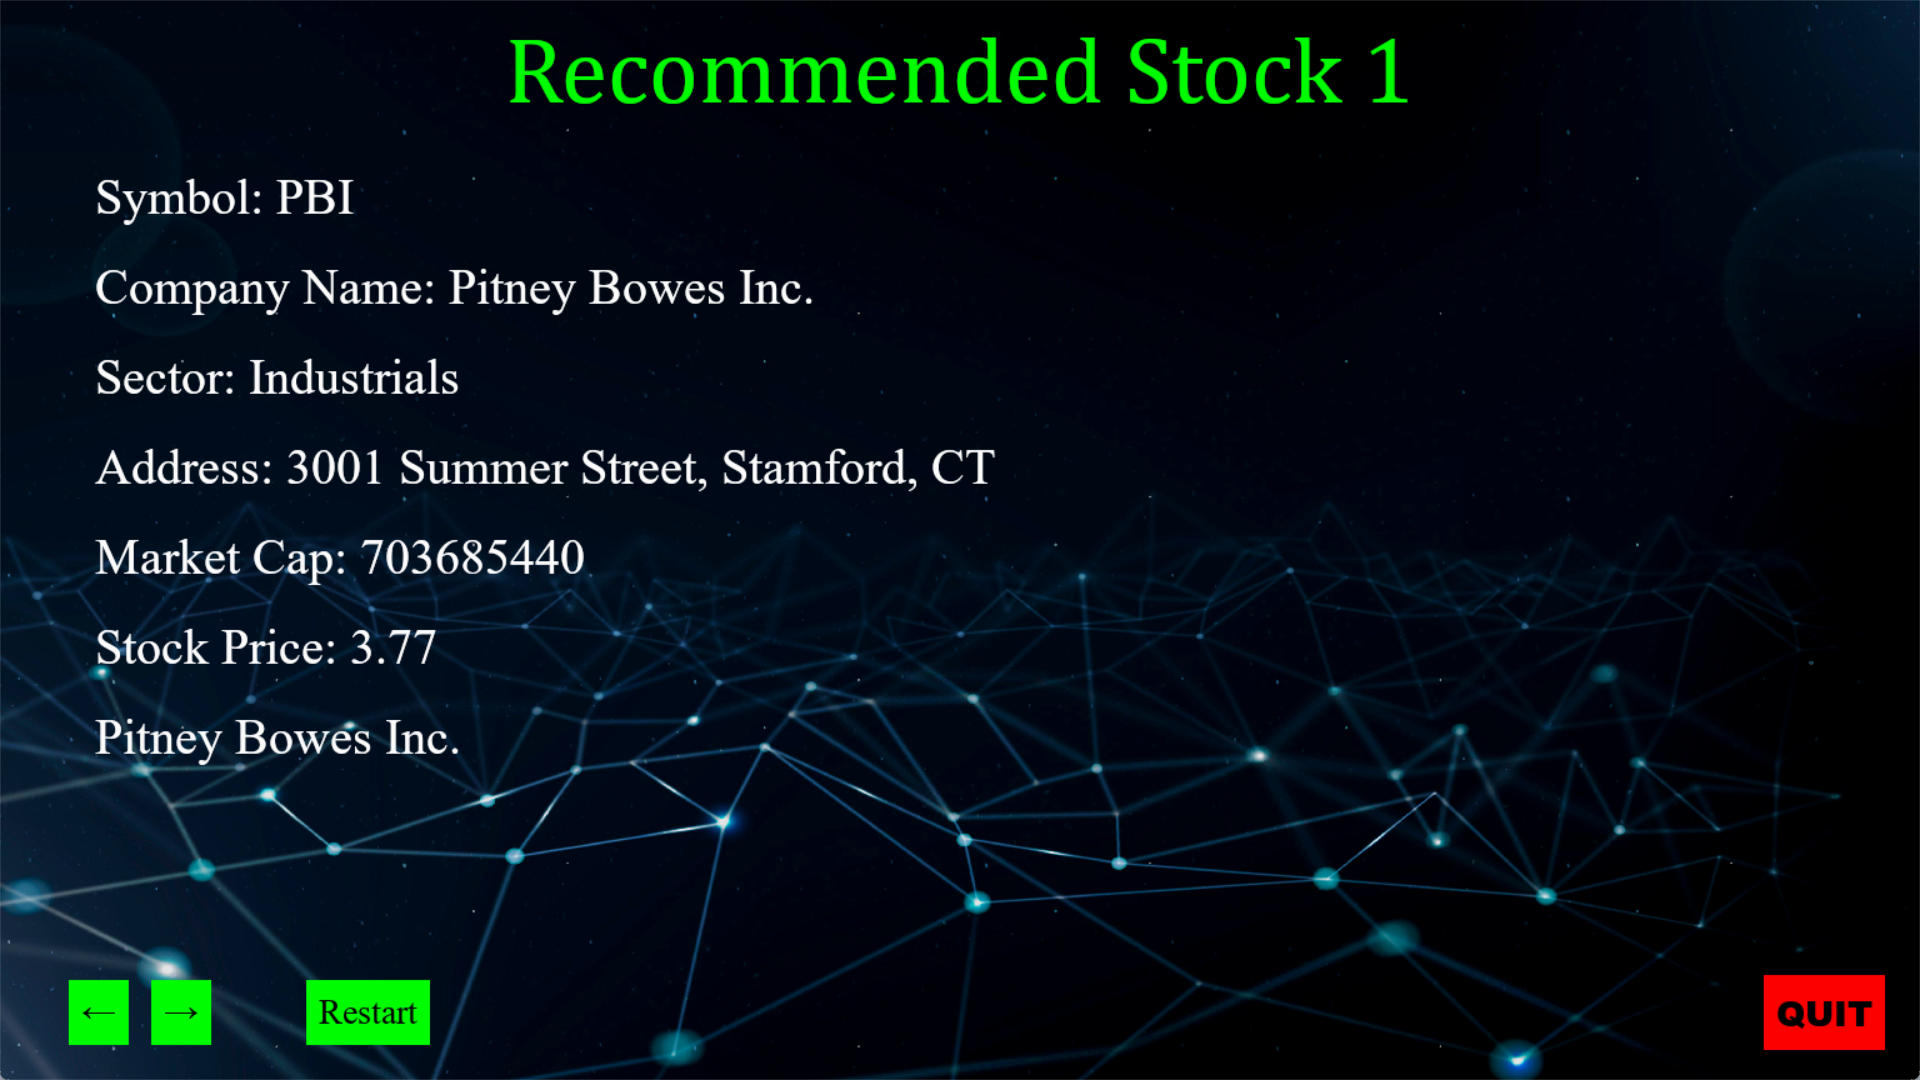
\includegraphics[width=\linewidth]{img/i.png}
  \caption{I}\label{fig:awesome_image1}
\endminipage\hfill
\minipage{0.24\textwidth}
  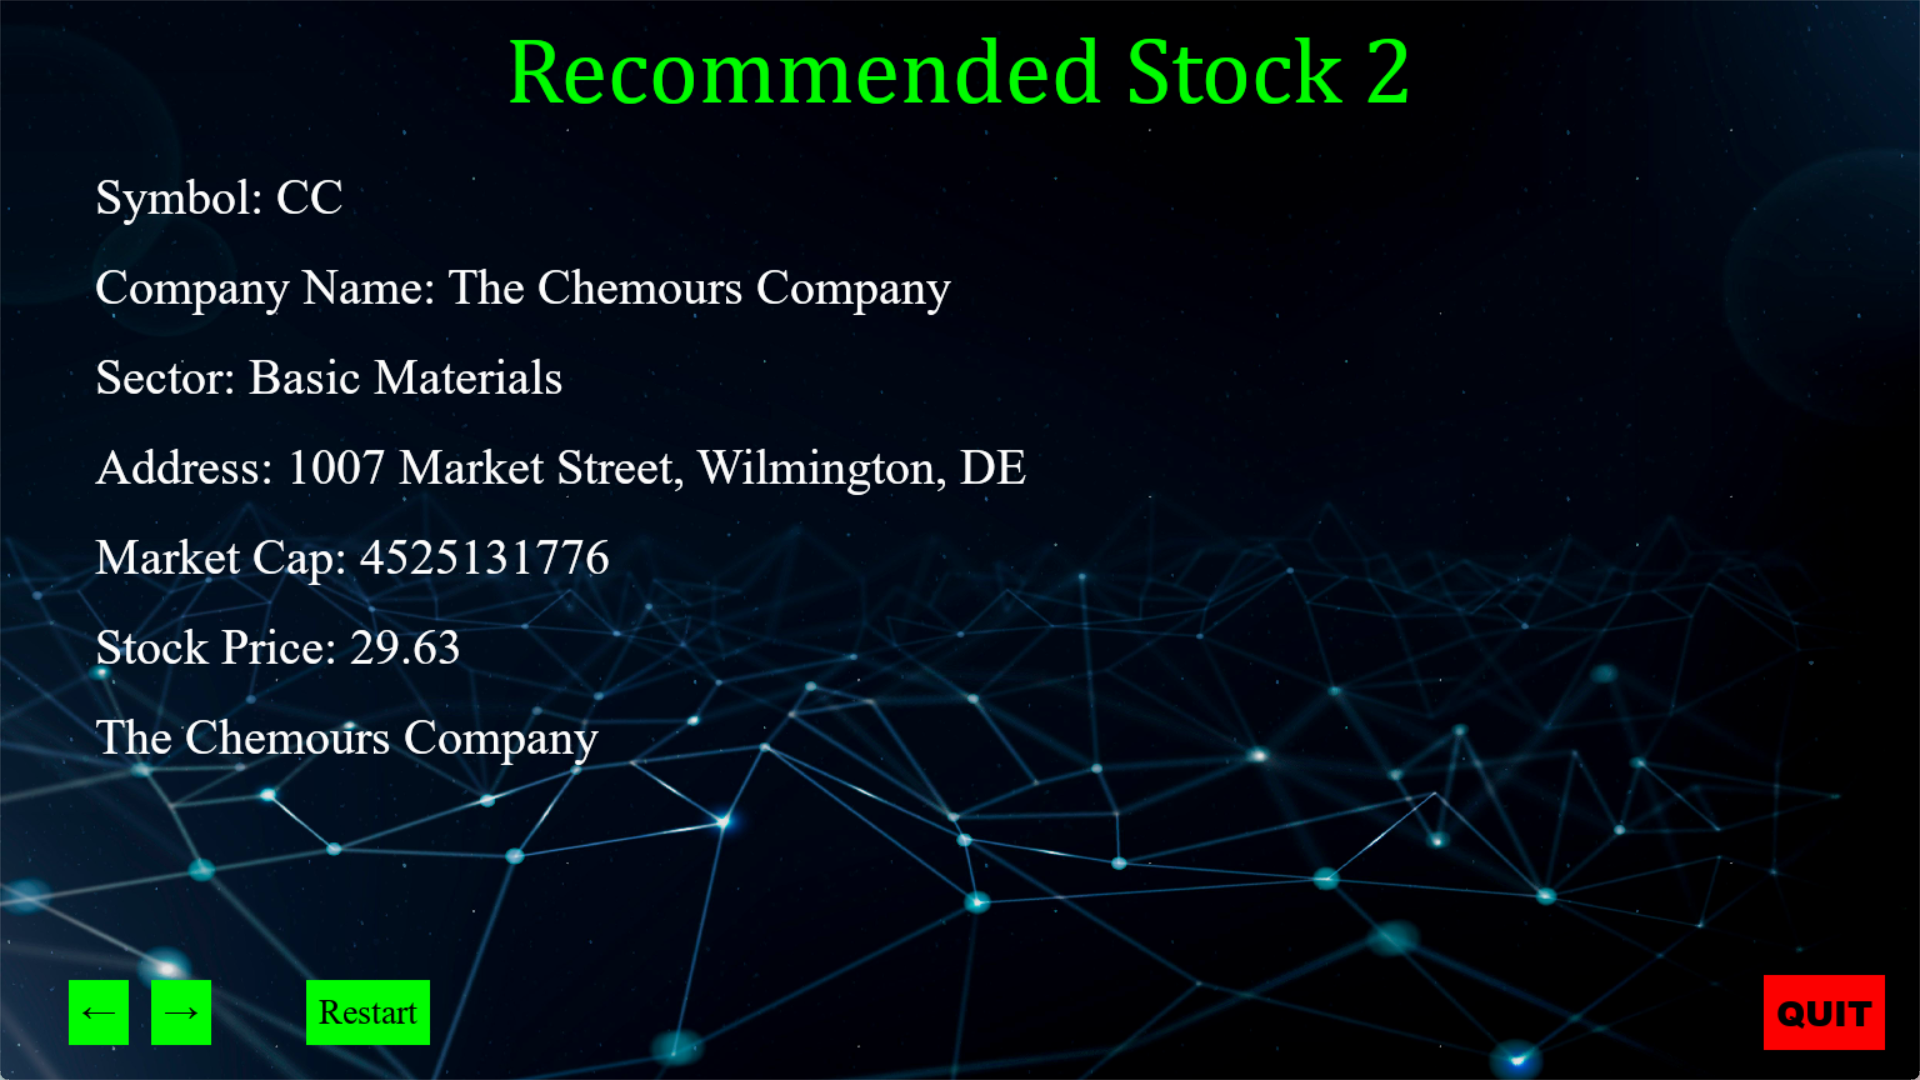
\includegraphics[width=\linewidth]{img/j.png}
  \caption{J}\label{fig:awesome_image2}
\endminipage\hfill
\end{figure}

\section*{Revised Project Plan}
\begin{quote}
\noindent
Our program achieves the project goal; it takes in the user’s preferences and outputs the best stocks for them to buy! It even has the ability to update the dataset to the most recent stock information, solving our project goal for the future too. All these components are delivered through an interactive and visually appealing user interface.
	
However, we still ran into several challenges during development. Some stocks from the dataset had missing values(in particular ESG scores), so we resorted to using the sector average value to fill in these gaps. However, this could lead to some stock misrepresentation from inaccurate score calculations. Then, the stock symbols are from our current csv file. This means that the stock symbols will not become updated in the case that new stocks get upgraded to large cap stocks or existing large cap stocks become downgraded to mid cap. We also had to learn how to webscrape from the current Yahoo websites to form our datasets. If these websites change their format, we’d have to update our code to properly extract the data again. Finally, we also had some time concerns over how long it took to web scrape the data.

Since our stock recommender is heavily dependent on the data set, it limits the types of stocks we can recommend to the user. Although it is possible to use web scraping to acquire a larger dataset with more stocks, the algorithm may not be as effective with a mix of different types of stocks. More specifically, our stock recommender is mainly built to recommend large cap stocks. It wouldn't necessarily be a problem if we incorporate stocks from other countries into our data set as long as they are large cap stocks. The problem arises if they are not large cap stocks. For example if we were to add penny stocks, our recommender would not be as nearly as accurate as our score values we use to recommend a stock would be all over the place and inconsistent as we designed the algorithm to focus on large cap stocks. Then, despite our efforts to create decision trees that divided the stocks over a large variety of user inputs, there are several instances where the user would get no recommended stocks based on their input criteria. 

Unfortunately, one thing we couldn’t adjust to the user’s screen size were the text sizes, as the font sizes had to be inputted manually while displaying texts. As a next step, we could try creating helper functions that adjust text sizes so we get a consistently sized display no matter the screen size. Another practical extension would be reducing the amount of cases where no stock is recommended. To do this, we could try calculating and adjusting our decision tree for a more even distribution of stocks, or increase the number of stocks in our dataset by web scraping from alternative sites(this approach would further increase the time to update our csv files though). Finally, we could also add the initially planned visual graph as an addition to our recommended stocks. Although it wouldn’t provide specific information, the graph would make a nice general overview between related stocks.
\end{quote}

\section*{References \& Acknowledgments}


\begin{itemize} 
\begin{refsection}
\item Mooney, P. (2023, January 16). Stock market data (NASDAQ, NYSE, $S\&P500$). Kaggle. 

\url{https://www.kaggle.com/datasets/paultimothymooney/stock-market-data}
\end{refsection}

\begin{refsection}
\item Pinkasovitch, A. (2022, August 2). How to pick a stock: Basic best practices for new investors. Investopedia.

\url{https://www.investopedia.com/articles/basics/11/how-to-pick-a-stock.asp}
\end{refsection}

\begin{refsection}
\item 5g networking technology background with blue digital line Free Vector. (2021, July 25). Freepik. 

\url{https://www.freepik.com/free-vector/5g-networking-technology-background-with-blue-digital-line_16406299.htm}

\end{refsection}

\begin{refsection}
\item Elmerraji, J. (2022, June 6). Analyze investments quickly with ratios. Investopedia. 

\url{https://www.investopedia.com/articles/stocks/06/ratios.asp}
\end{refsection}

\begin{refsection}
\item Stock market 101. What is Stock Market? (n.d.).

\url{https://www.td.com/ca/en/investing/direct-investing/articles/what-is-stock-market}.
\end{refsection}

\begin{refsection}
\item Wilkins, G. (2022, November 10). 6 basic financial ratios and what they reveal. Investopedia. 

\url{https://www.investopedia.com/financial-edge/0910/6-basic-financial-ratios-and-what-they-tell-you.aspx}
\end{refsection}

\begin{refsection}
\item Stock Dataset

\url{https://query2.finance.yahoo.com/v10/finance/quoteSummary/+stock+?modules=summaryProfile%2CsummaryDetail%2CesgScores%2CincomeStatementHistory%2CdefaultKeyStatistics%2CfinancialData%2CbalanceSheetHistory%2Cprice}
\end{refsection}

\end{itemize}
\begin{center}
    Made with \LaTeX 
\end{center}
\end{document}